\documentclass[14pt, a4paper]{extarticle}

\usepackage[utf8]{inputenc}
\usepackage[T1]{fontenc}
\usepackage{amsmath}
\usepackage{amssymb}
\usepackage{graphicx}
\usepackage[left=2.00cm, right=2.00cm, top=2.00cm, bottom=2.00cm]{geometry}
\usepackage[russian]{babel}

\usepackage{setspace}
\usepackage{fancyhdr}

\graphicspath{{img/}}

\RequirePackage{caption}
\captionsetup[figure]{justification=centering,name=Рисунок,labelsep=endash}

\usepackage{indentfirst}

\usepackage{float}

\begin{document}
	\onehalfspacing
	\begin{titlepage}
	\begin{center}
		\begin{small}
			\textbf{Министерство науки и высшего образования Российской Федерации}

			ФЕДЕРАЛЬНОЕ ГОСУДАРСТВЕННОЕ АВТОНОМНОЕ ОБРАЗОВАТЕЛЬНОЕ УЧРЕЖДЕНИЕ ВЫСШЕГО ОБРАЗОВАНИЯ
			
			\textbf{<<НАЦИОНАЛЬНЫЙ ИССЛЕДОВАТЕЛЬСКИЙ УНИВЕРСИТЕТ ИТМО>>}
		\end{small}
		
		\vspace{8em}
		
		Отчет по лабораторной работе №4
		
		СИНТЕЗ ОПТИМАЛЬНОГО УПРАВЛЕНИЯ. ПРИНЦИП МАКСИМУМА
		
		По дисциплине <<Оптимальное управление>>
	\end{center}
	
	\vspace{8em}
	
	\begin{flushright}
		Выполнил:\\
		студент группы R42331c\\
		Манахов~С.П.
		
		\vspace{1em}
		
		Преподаватель:\\
		Парамонов~А.В.
	\end{flushright}

	\vfill
	
	\begin{center}
		\small
		Санкт-Петербург\\
		2022 г.\\
	\end{center}
\end{titlepage}
	\setcounter{page}{2}
	
	\section*{Задание}
	
	\begin{enumerate}
		\item Дан линейный объект управления:
		$$\dot{x}=Ax+bu, x(0)$$
		и критерий качества:
		$$J = \int\limits_0^\infty x^T(t)Qx(t) + ru^2(t)dt$$
		Построить оптимальный регулятор с помощью метода динамического программирования Беллмана и промоделировать его работу на заданном интервале времени;
		\item Параметры $A,b,Q,r$ взять из задания~2. Начальные условия выбрать $x(0)=[1, 0]^T$. Построить графики управления $u$, переменных состояния $x_1,x_2$ и критерия $J$;
		\item Построить критерий при отклонениях параметров регулятора от оптимальных значений.
	\end{enumerate}
	\begin{table}[H]
		\centering
		\begin{tabular}{|c|c|c|c|c|}
			\hline
			Вариант & Матрица $A$ & Матрица $b$ & Матрица $Q$ & Параметр $r$ \\\hline
			9 & 
			$\left[
			\begin{matrix}
				0 & 1 \\
				0 & 0 
			\end{matrix}
			\right]$
			& 
			$\left[
			\begin{matrix}
				0 \\ 5
			\end{matrix}
			\right]$
			& 
			$\left[
			\begin{matrix}
				2 & 0 \\
				0 & 3 
			\end{matrix}
			\right]$
			& 4 \\\hline
		\end{tabular}
	\end{table}
	
	\newpage
	
	\section*{Описание работы}
	
	Функция Беллмана в данном случае равняется:
	$$S(x(\tau),\tau) = \underset{u(t)}{min}\left[\int\limits_\tau^\infty x^T(t)Qx(t) + ru^2(t)dt\right]$$
	
	Составим уравнение Беллмана:
	$$\underset{u(t)}{min}\left[x^T(t)Qx(t) + ru^2(t) + \frac{\partial S}{\partial x}\left(Ax + Bu\right)\right] = 0$$
	
	Тогда закон оптимального управления:
	$$\begin{matrix}
		x^T(t)Qx(t) + ru^2(t) + \frac{\partial S}{\partial x}\left(Ax + Bu\right) = 0 \\
		\frac{\partial}{\partial u}\left[x^T(t)Qx(t) + ru^2(t) + \frac{\partial S}{\partial x}\left(Ax + Bu\right)\right] = 0
	\end{matrix}$$
	
	Подставим параметры в соответствии с вариантом задания:
	$$2x_1^2 + 3x_2^2 +4u^2 + \frac{\partial S}{\partial x_1}x_2 + \frac{\partial S}{\partial x_2}5u = 0$$
	
	Выберем функцию Беллмана:
	$$S = \psi_1x_1^2 + \psi_{12}x_1x_2 + \psi_2x_2^2$$
	
	Подставим частные производные $\frac{\partial}{\partial x_1}, \frac{\partial}{\partial x_2}$, а затем найдем частную производную по управляющему сигналу $u$:
	$$8u + 5\psi_{12}x_1 + 10\psi_2x_2 = 0$$
	
	Откуда:
	$$u = -\frac{5}{8}\psi_{12}x_1 - \frac{10}{8}\psi_2x_2$$
	
	После всех подстановок и сокращений получаем систему уравнений:
	$$\begin{cases}
		2 - \frac{100}{64}\psi_{12}^2 = 0 \\
		3 + \psi_{12} - \frac{400}{64}\psi_2^2 = 0 \\
		2\psi_1 - \frac{400}{64}\psi_{12}\psi_2 = 0
	\end{cases}$$
	
	Откуда:
	$$\begin{matrix}
		\psi_{12} = \sqrt{\frac{128}{100}}\\
		\psi_2 = \sqrt{\frac{64}{400}\left(3 + \sqrt{\frac{128}{100}}\right)}
	\end{matrix}$$
	
	Полученная при помощи пакета \textit{MATLAB~Simulink} система представлена на рисунках \ref{fig:system}--\ref{fig:MATLAB-Function}.
	
	\begin{figure}[H]
		\centering
		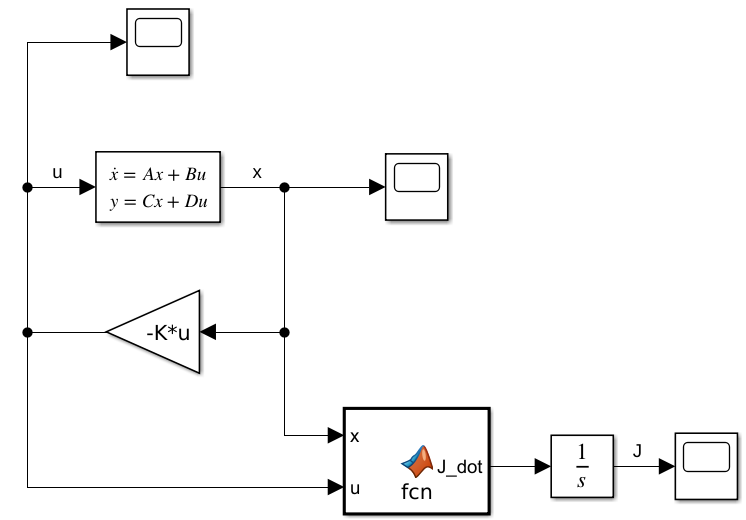
\includegraphics[width=0.6\textwidth]{system}
		\caption{Замкнутая система}
		\label{fig:system}
	\end{figure}
	
	\begin{figure}[H]
		\centering
		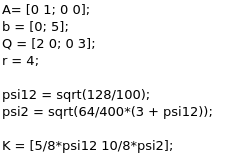
\includegraphics{properties}
		\caption{Параметры системы}
		\label{fig:properties}
	\end{figure}
	
	\begin{figure}[H]
		\centering
		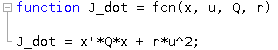
\includegraphics{MATLAB-Function}
		\caption{Блок MATLAB-Function}
		\label{fig:MATLAB-Function}
	\end{figure}
	
	Произведем моделирование системы при начальных условиях $x(0)=[1,0]^T$. Полученные графики представлены на рисунках \ref{fig:x-2}--\ref{fig:J-2}.
	
	\begin{figure}[H]
		\centering
		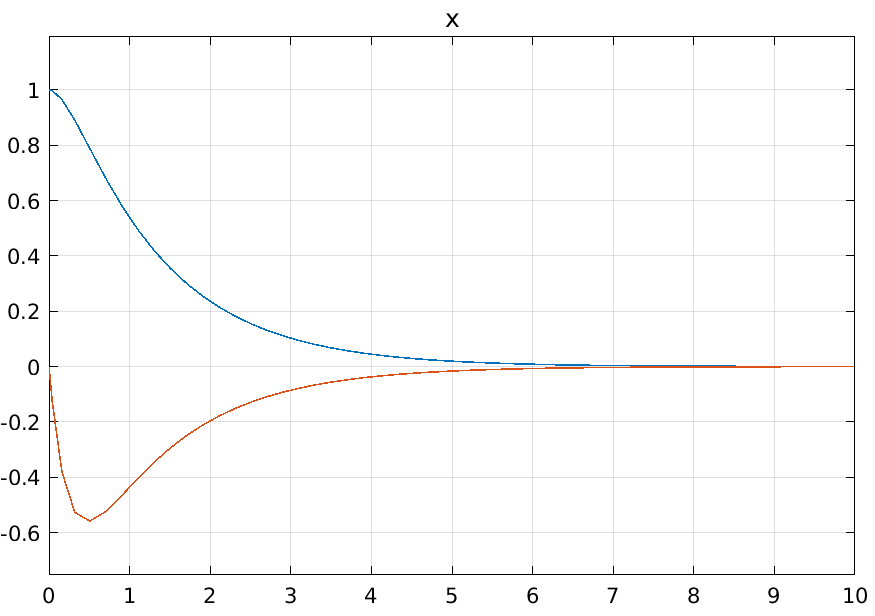
\includegraphics[width=0.59\textwidth]{x-2}
		\caption{Вектор состояния системы $x$ при $x(0)=[1,0]^T$}
		\label{fig:x-2}
	\end{figure}
	
	\begin{figure}[H]
		\centering
		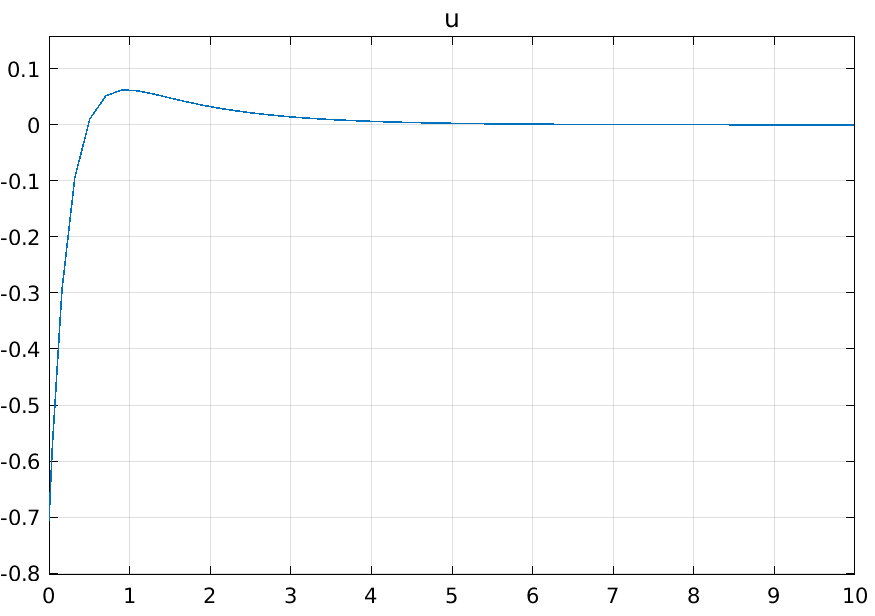
\includegraphics[width=0.59\textwidth]{u-2}
		\caption{Управляющий сигнал $u$ при $x(0)=[1,0]^T$}
		\label{fig:u-2}
	\end{figure}
	
	\begin{figure}[H]
		\centering
		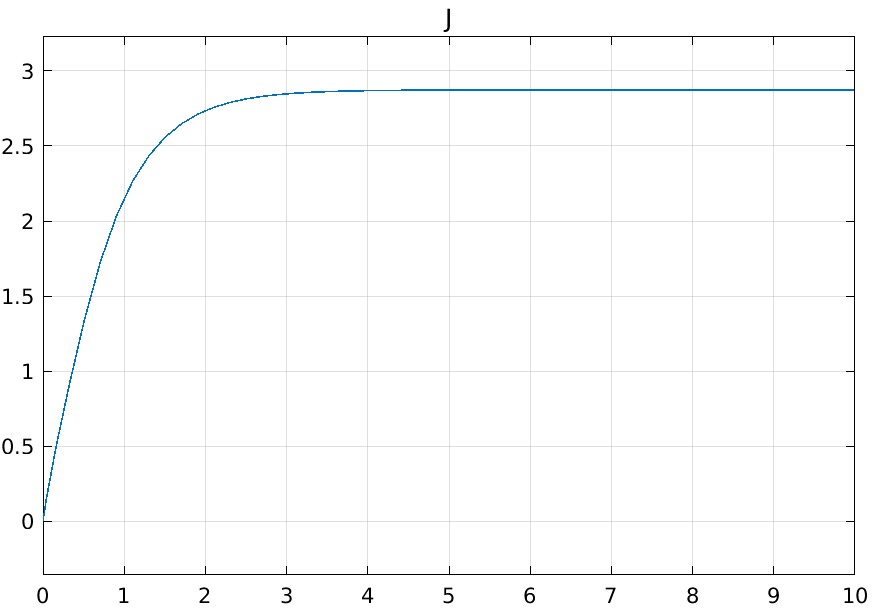
\includegraphics[width=0.59\textwidth]{J-2}
		\caption{Критерий качества $J$ при $x(0)=[1,0]^T$}
		\label{fig:J-2}
	\end{figure}
	
	Графики идентичны тем, что получились при выполнении задания~2. Матрица коэффициентов обратной связи $K$ тоже совпадает:
	$$K = \left[\begin{matrix}
		0,7071 & 1,0163
	\end{matrix}\right]$$
	
	Теперь незначительно отклоним расчетное значение $K$ в положительную сторону $K+1$. Полученные графики представлены на рисунках \ref{fig:x-3-plus}--\ref{fig:J-3-plus}.
	
	\begin{figure}[H]
		\centering
		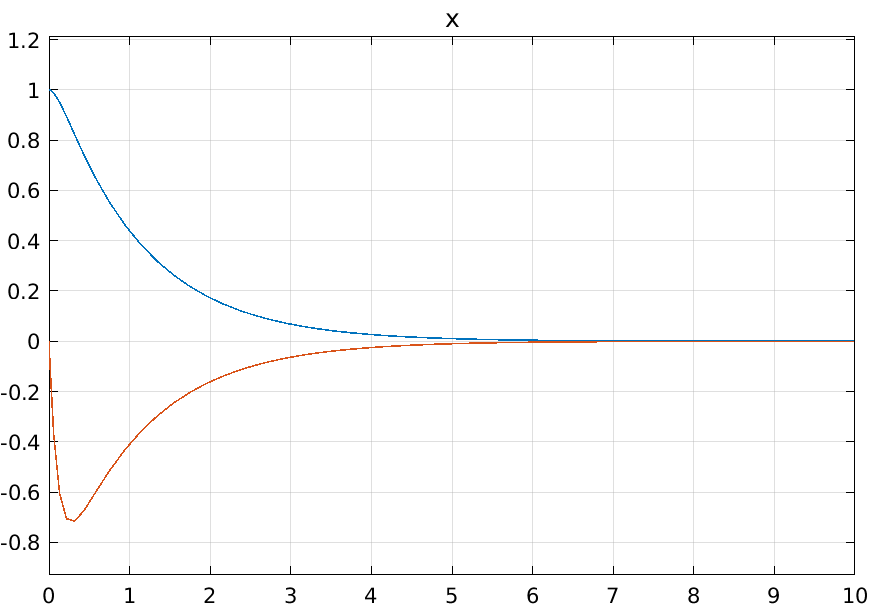
\includegraphics[width=0.59\textwidth]{x-3-plus}
		\caption{Вектор состояния системы $x$ при отклонении $K+1$}
		\label{fig:x-3-plus}
	\end{figure}
	
	\begin{figure}[H]
		\centering
		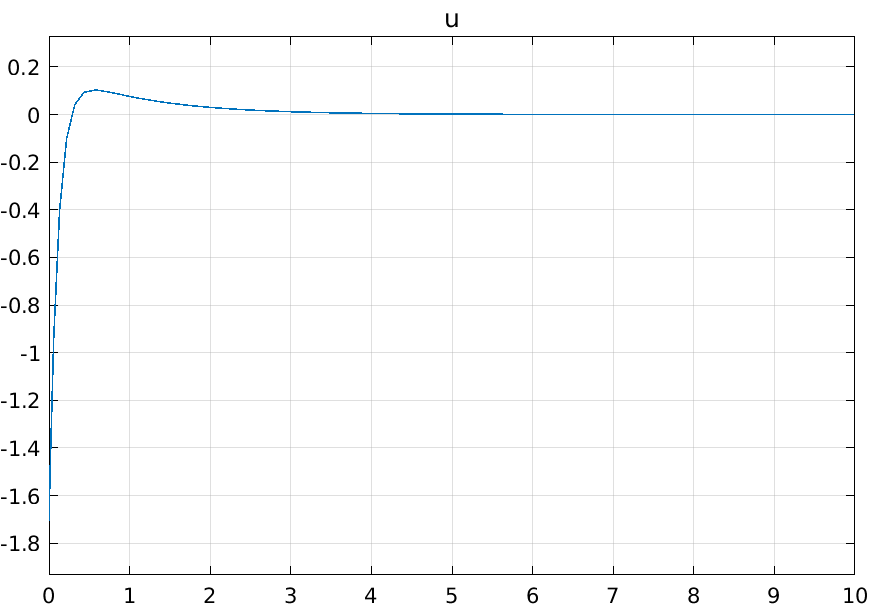
\includegraphics[width=0.59\textwidth]{u-3-plus}
		\caption{Управляющий сигнал $u$ при отклонении $K+1$}
		\label{fig:u-3-plus}
	\end{figure}
	
	\begin{figure}[H]
		\centering
		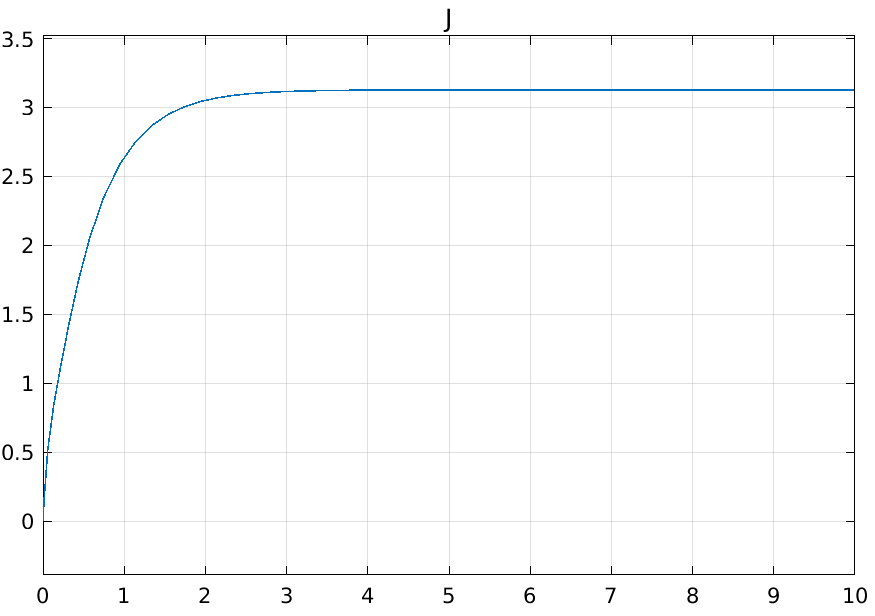
\includegraphics[width=0.59\textwidth]{J-3-plus}
		\caption{Критерий качества $J$ при отклонении $K+1$}
		\label{fig:J-3-plus}
	\end{figure}
	
	Время переходного процесса практически не изменилось, но увеличились предельные значения управляющего сигнала $u$. Также увеличилось установившееся значение критерия качества $J$.
	
	При отрицательном отклонении $K-1$ система расходится, поэтому промоделируем систему при $K-0,5$. Полученные графики представлены на рисунках \ref{fig:x-3-minus}--\ref{fig:J-3-minus}.
	
	\begin{figure}[H]
		\centering
		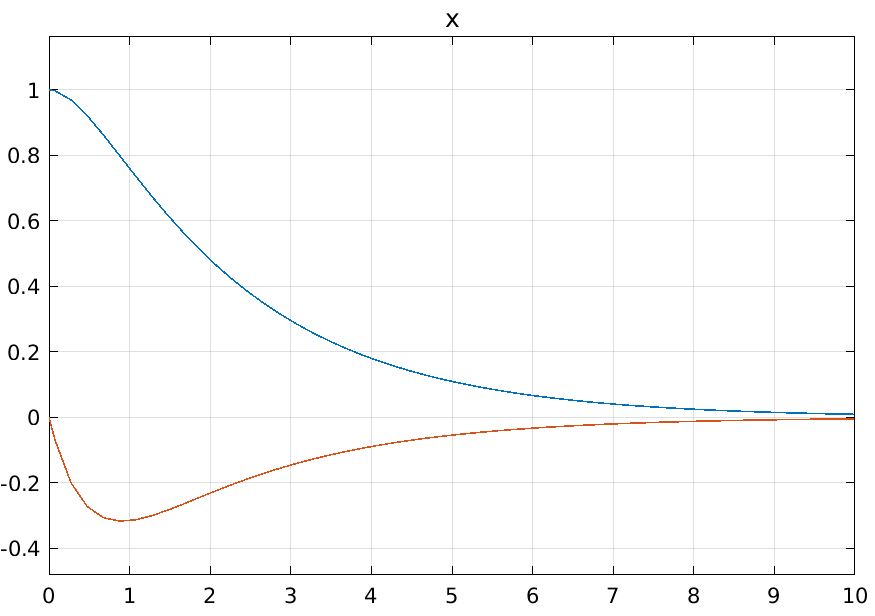
\includegraphics[width=0.59\textwidth]{x-3-minus}
		\caption{Вектор состояния системы $x$ при отклонении $K-0,5$}
		\label{fig:x-3-minus}
	\end{figure}
	
	\begin{figure}[H]
		\centering
		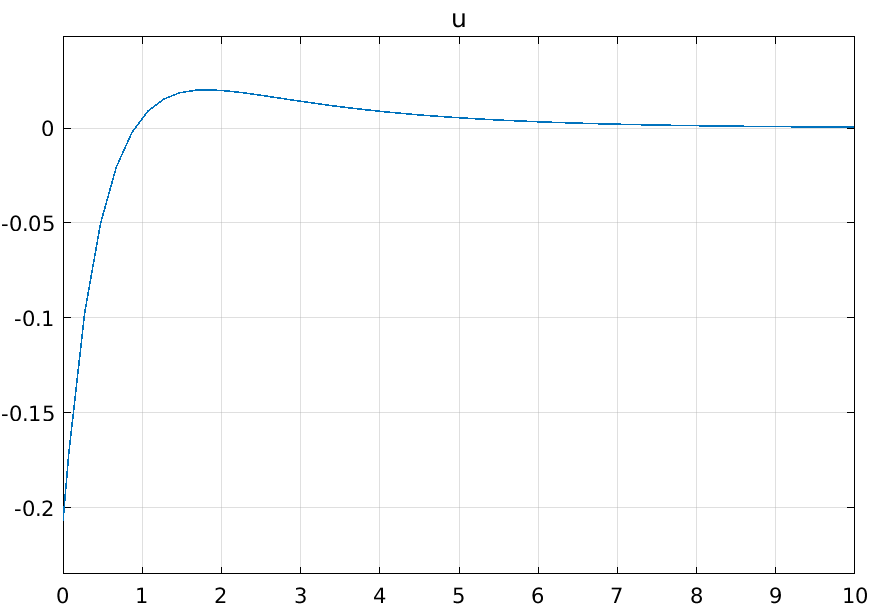
\includegraphics[width=0.59\textwidth]{u-3-minus}
		\caption{Управляющий сигнал $u$ при отклонении $K-0,5$}
		\label{fig:u-3-minus}
	\end{figure}
	
	\begin{figure}[H]
		\centering
		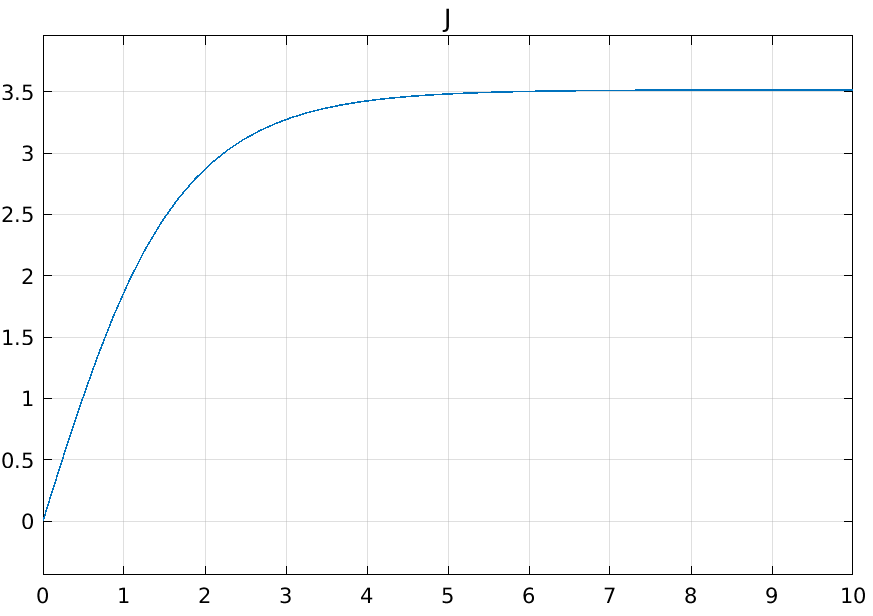
\includegraphics[width=0.59\textwidth]{J-3-minus}
		\caption{Критерий качества $J$ при отклонении $K-0,5$}
		\label{fig:J-3-minus}
	\end{figure}
	
	Время переходного процесса и установившееся значение критерия качества $J$ увеличились.
	
	\newpage
	
	\section*{Вывод}
	
	В данном случае критерий качества задавался с нулевым терминантом, что полностью соответствует критерию качества из задания~2. Так как полученные результаты совпадают, можно сделать вывод об оптимальности управления.
	
\end{document}